\qrchapter{https://forgottenpillar.com/rsc/en-fp-chapter23}{The great apostasy is soon to be realized} \label{chap:apostasy}


\qrchapter{https://forgottenpillar.com/rsc/en-fp-chapter23}{Ukengeufu mkuu utakuja kutimizwa hivi karibuni} \label{chap:apostasy}


In 1903, when the Living Temple was published and instigated the controversy over the \emcap{personality of God}, Sister White was faithfully obeying the command of the Great Commander. She was called by the words “\textit{Meet it!}” She faced this controversy by writing numerous letters to many people in the field. In these letters, we trace the prophetic insight of the future of the Seventh-day Adventist Church.


Mnamo 1903, wakati The Living Temple lilipochapishwa na kuanzisha mabishano juu ya \emcap{Umbile la Mungu}, Dada White alikuwa akitii kwa uaminifu amri ya Kamanda Mkuu. Aliitwa kwa maneno “\textit{Kutana nayo!}” Alikumbana na utata huu kwa kuandika barua nyingi kwa watu wengi waliokuwa katika utumishi maeneo pote. Katika barua hizi, tunafuatilia ufahamu wa kinabii wa mustakabali wa Kanisa la Waadventista Wasabato.


One example is the correspondence between Sister White and her son William White. On November 26, 1905, there was a great Health Conference in College View Nebraska, where many medical missionary workers met together. William White was there and he had a short, 30-minute public talk. Afterwards, he wrote a letter to his mother regarding his impressions from the conference. Here is part of that letter:


Mfano mmoja ni mawasiliano kati ya Dada White na mwanawe William White. Mnamo Novemba 26, 1905, kulikuwa na Kongamano kubwa la Afya katika College View Nebraska, ambapo wafanyakazi wengi wa kimisionari wa matibabu walikutana pamoja. William White alikuwepo na alikuwa na muda mfupi, hotuba ya watu wote ya dakika 30. Baadaye, aliandika barua kwa mama yake kuhusu maoni yake kutoka katika mkutano huo. Hapa kuna sehemu ya barua hiyo:


\others{College View, Ne. – Tuesday, November 28, 1905; Author: William C. White} \\
\others{Nov. 28, 1905.} \\
\others{Mrs. E. G. White, Sanitarium, Cala.}


\others{College View, Ne. – Jumanne, Novemba 28, 1905; Mwandishi: William C. White} \\
\others{Novemba 28, 1905.} \\
\others{Bi. E. G. White, Sanitarium, Cala.}


\othersnogap{...Sabbath morning I had opportunity to speak about thirty minutes. In my remarks I refered to the history of the Christian church. They began with pure principles, but through the attacks of Satan they became backslidden and departed from those principles. \textbf{I pointed out that the only hope for the S. D. A. church was to \underline{adhear to first principles}}. \textbf{I then referred to the order in which the enemy is attacking our work. His first effort was to destroy union and establish separation. His next work was to weaken our reverence for the Sabbath, then to weaken our faith in the Sanctuary service, then \underline{to break our confidence in the Spirit of Prophecy}, then to \underline{confuse our conception regarding a personal God}}.}[Letter from W. C. White to E. G. White, November 28, 1905.][http://ellenwhite.org/content/correspondence/incoming/43292pdf]


\othersnogap{...Sabato asubuhi nilipata nafasi ya kuzungumza kama dakika thelathini. Katika maelezo yangu nilirejelea kwa historia ya kanisa la Kikristo. Walianza na kanuni safi, lakini kupitia mashambulizi ya Shetani wakarudi nyuma na kuziacha kanuni hizo. \textbf{Nilielekeza kwamba tumaini pekee kwa kanisa la S. D. A. lilikuwa \underline{kuzingatia kanuni za kwanza}}. \textbf{Mimi basi narejelea mpangilio ambao adui anashambulia kazi yetu. Juhudi zake za kwanza zilikuwa kuharibu muungano na kuanzisha utengano. Kazi yake iliyofuata ilikuwa kudhoofisha heshima yetu kwa ajili ya Sabato, kisha kudhoofisha imani yetu katika huduma ya Patakatifu, kisha \underline{kuvunja imani yetu katika Roho wa Unabii}, kisha \underline{kuchanganya dhana yetu kuhusu Mungu wa kibinafsi}}.}[Letter from W. C. White to E. G. White, November 28, 1905.][http://ellenwhite.org/content/correspondence/incoming/43292pdf]


\begin{figure}
    \centering
    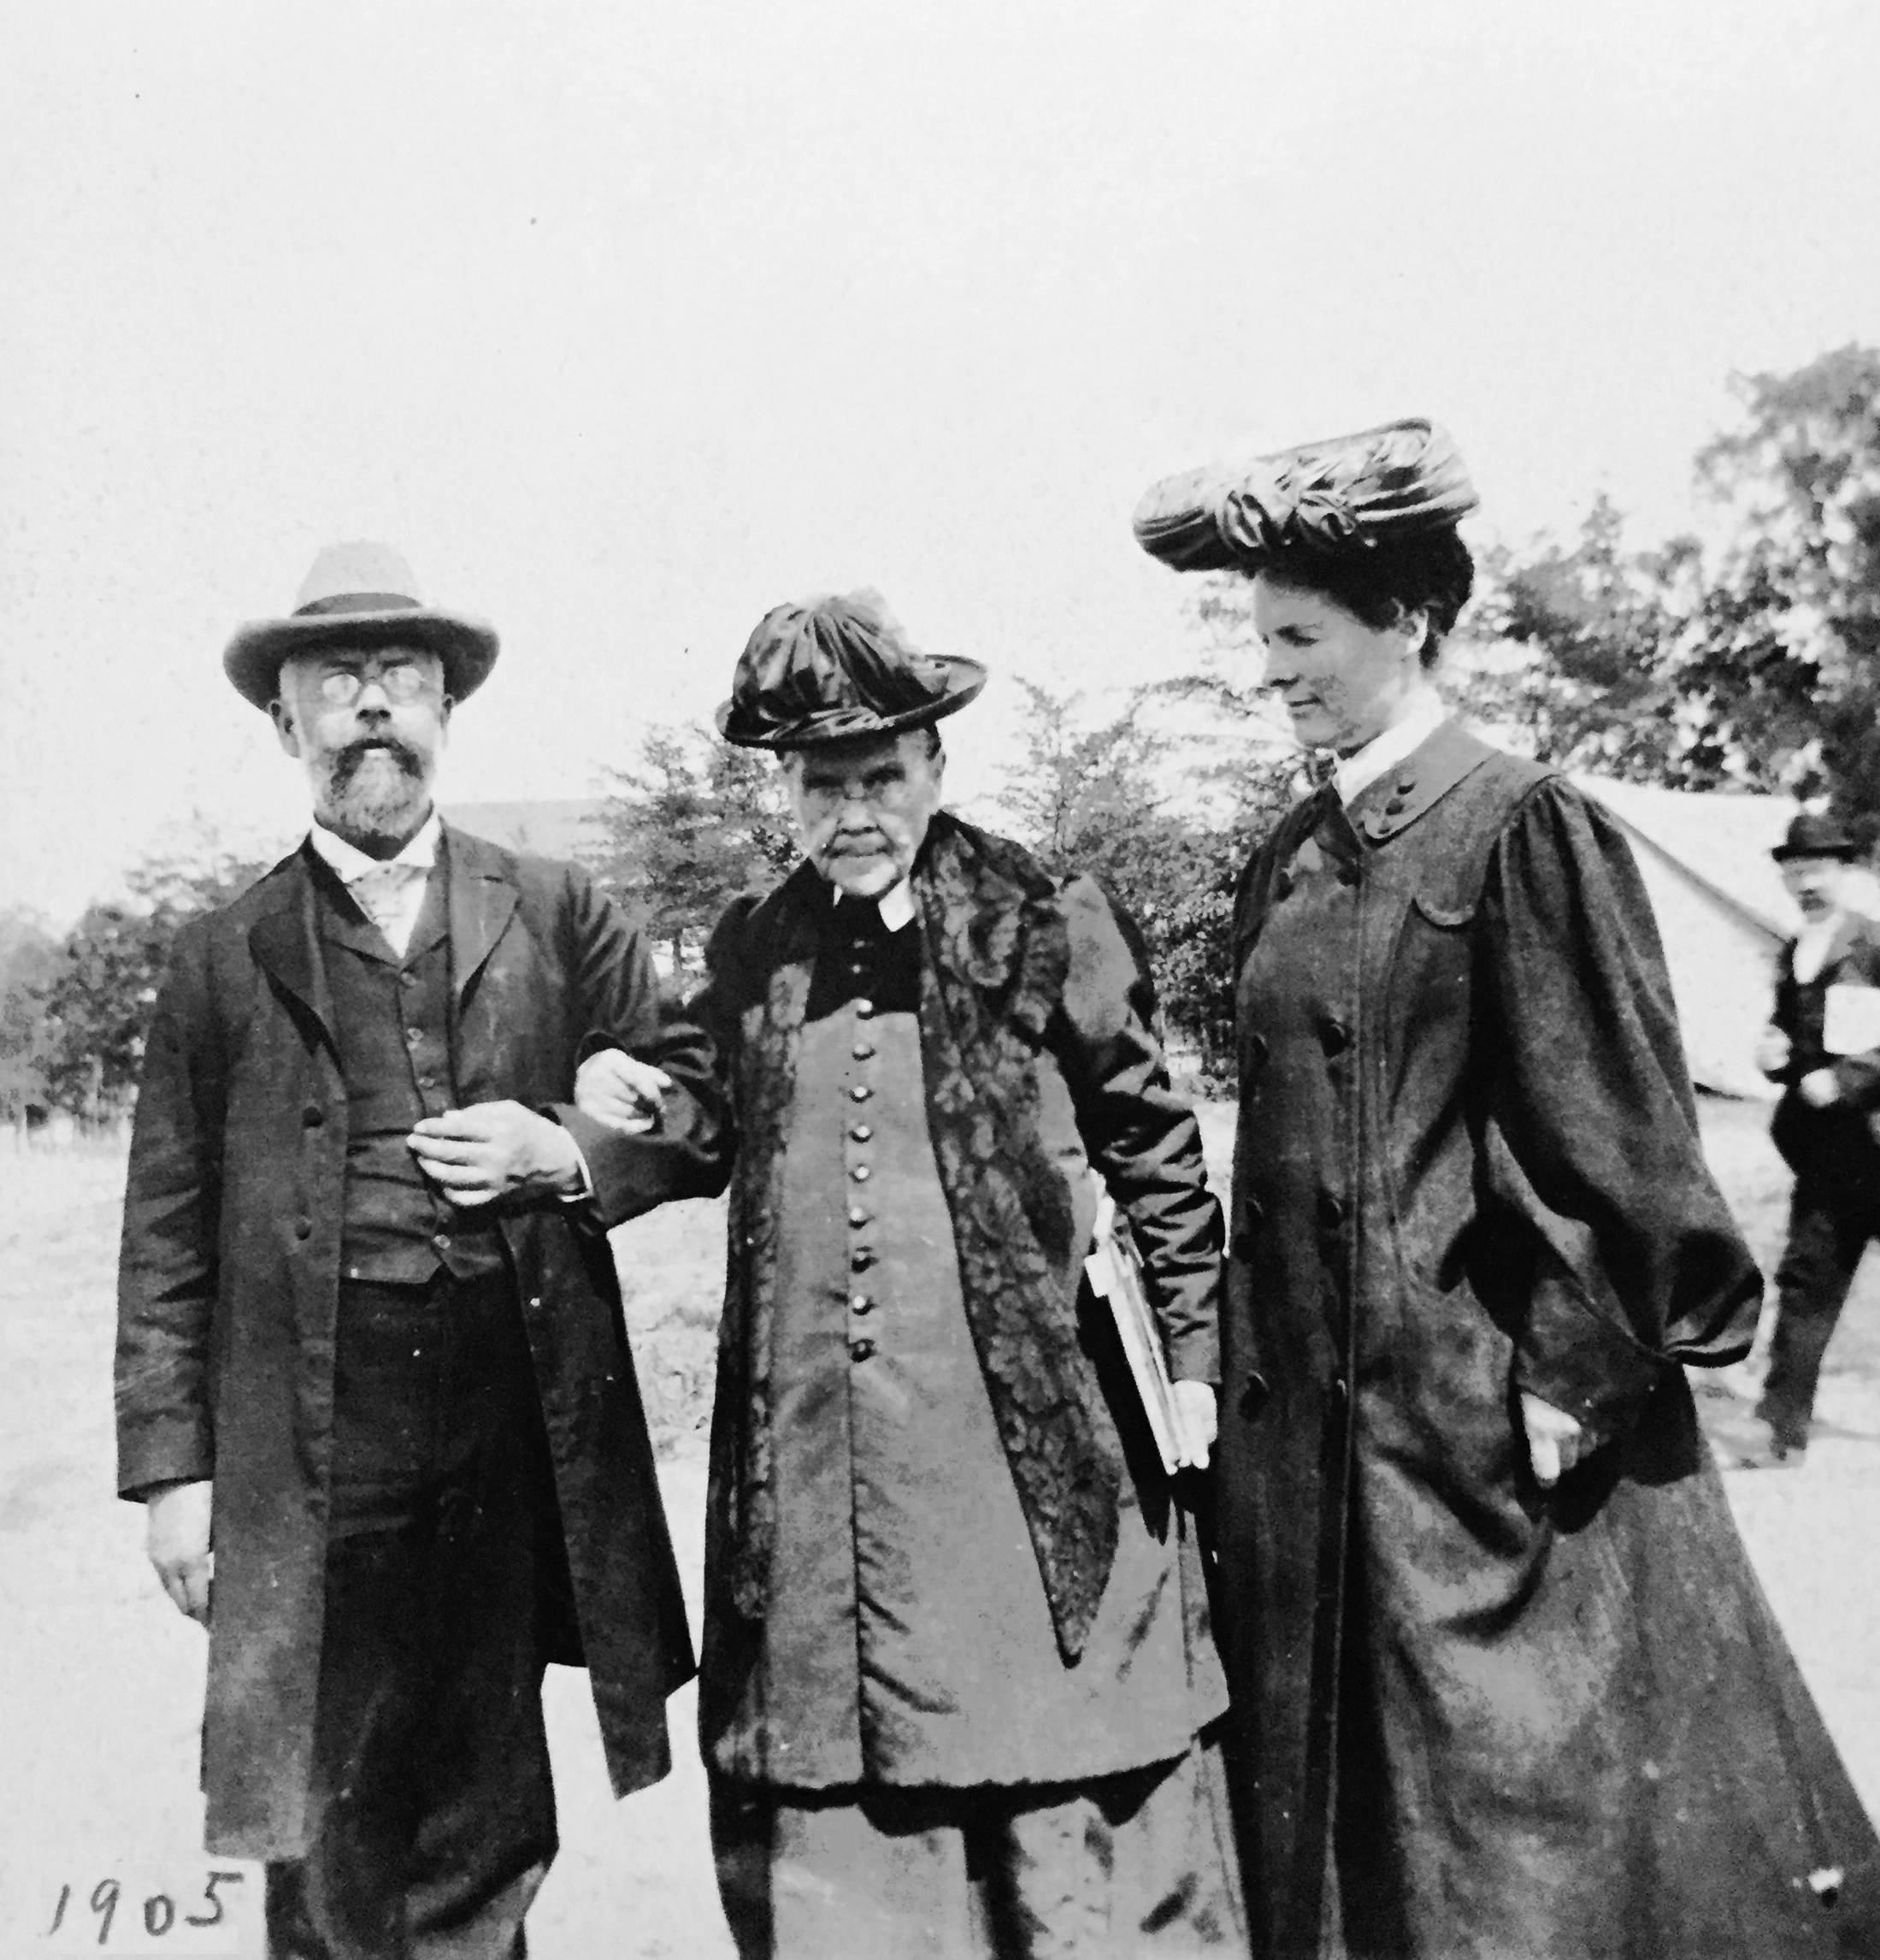
\includegraphics[width=1\linewidth]{images/william-ellen-white-1905.jpg}
    \caption*{William C. White and Ellen G. White, 1905}
    \label{fig:w-e-white}
\end{figure}


\begin{figure}
    \centering
    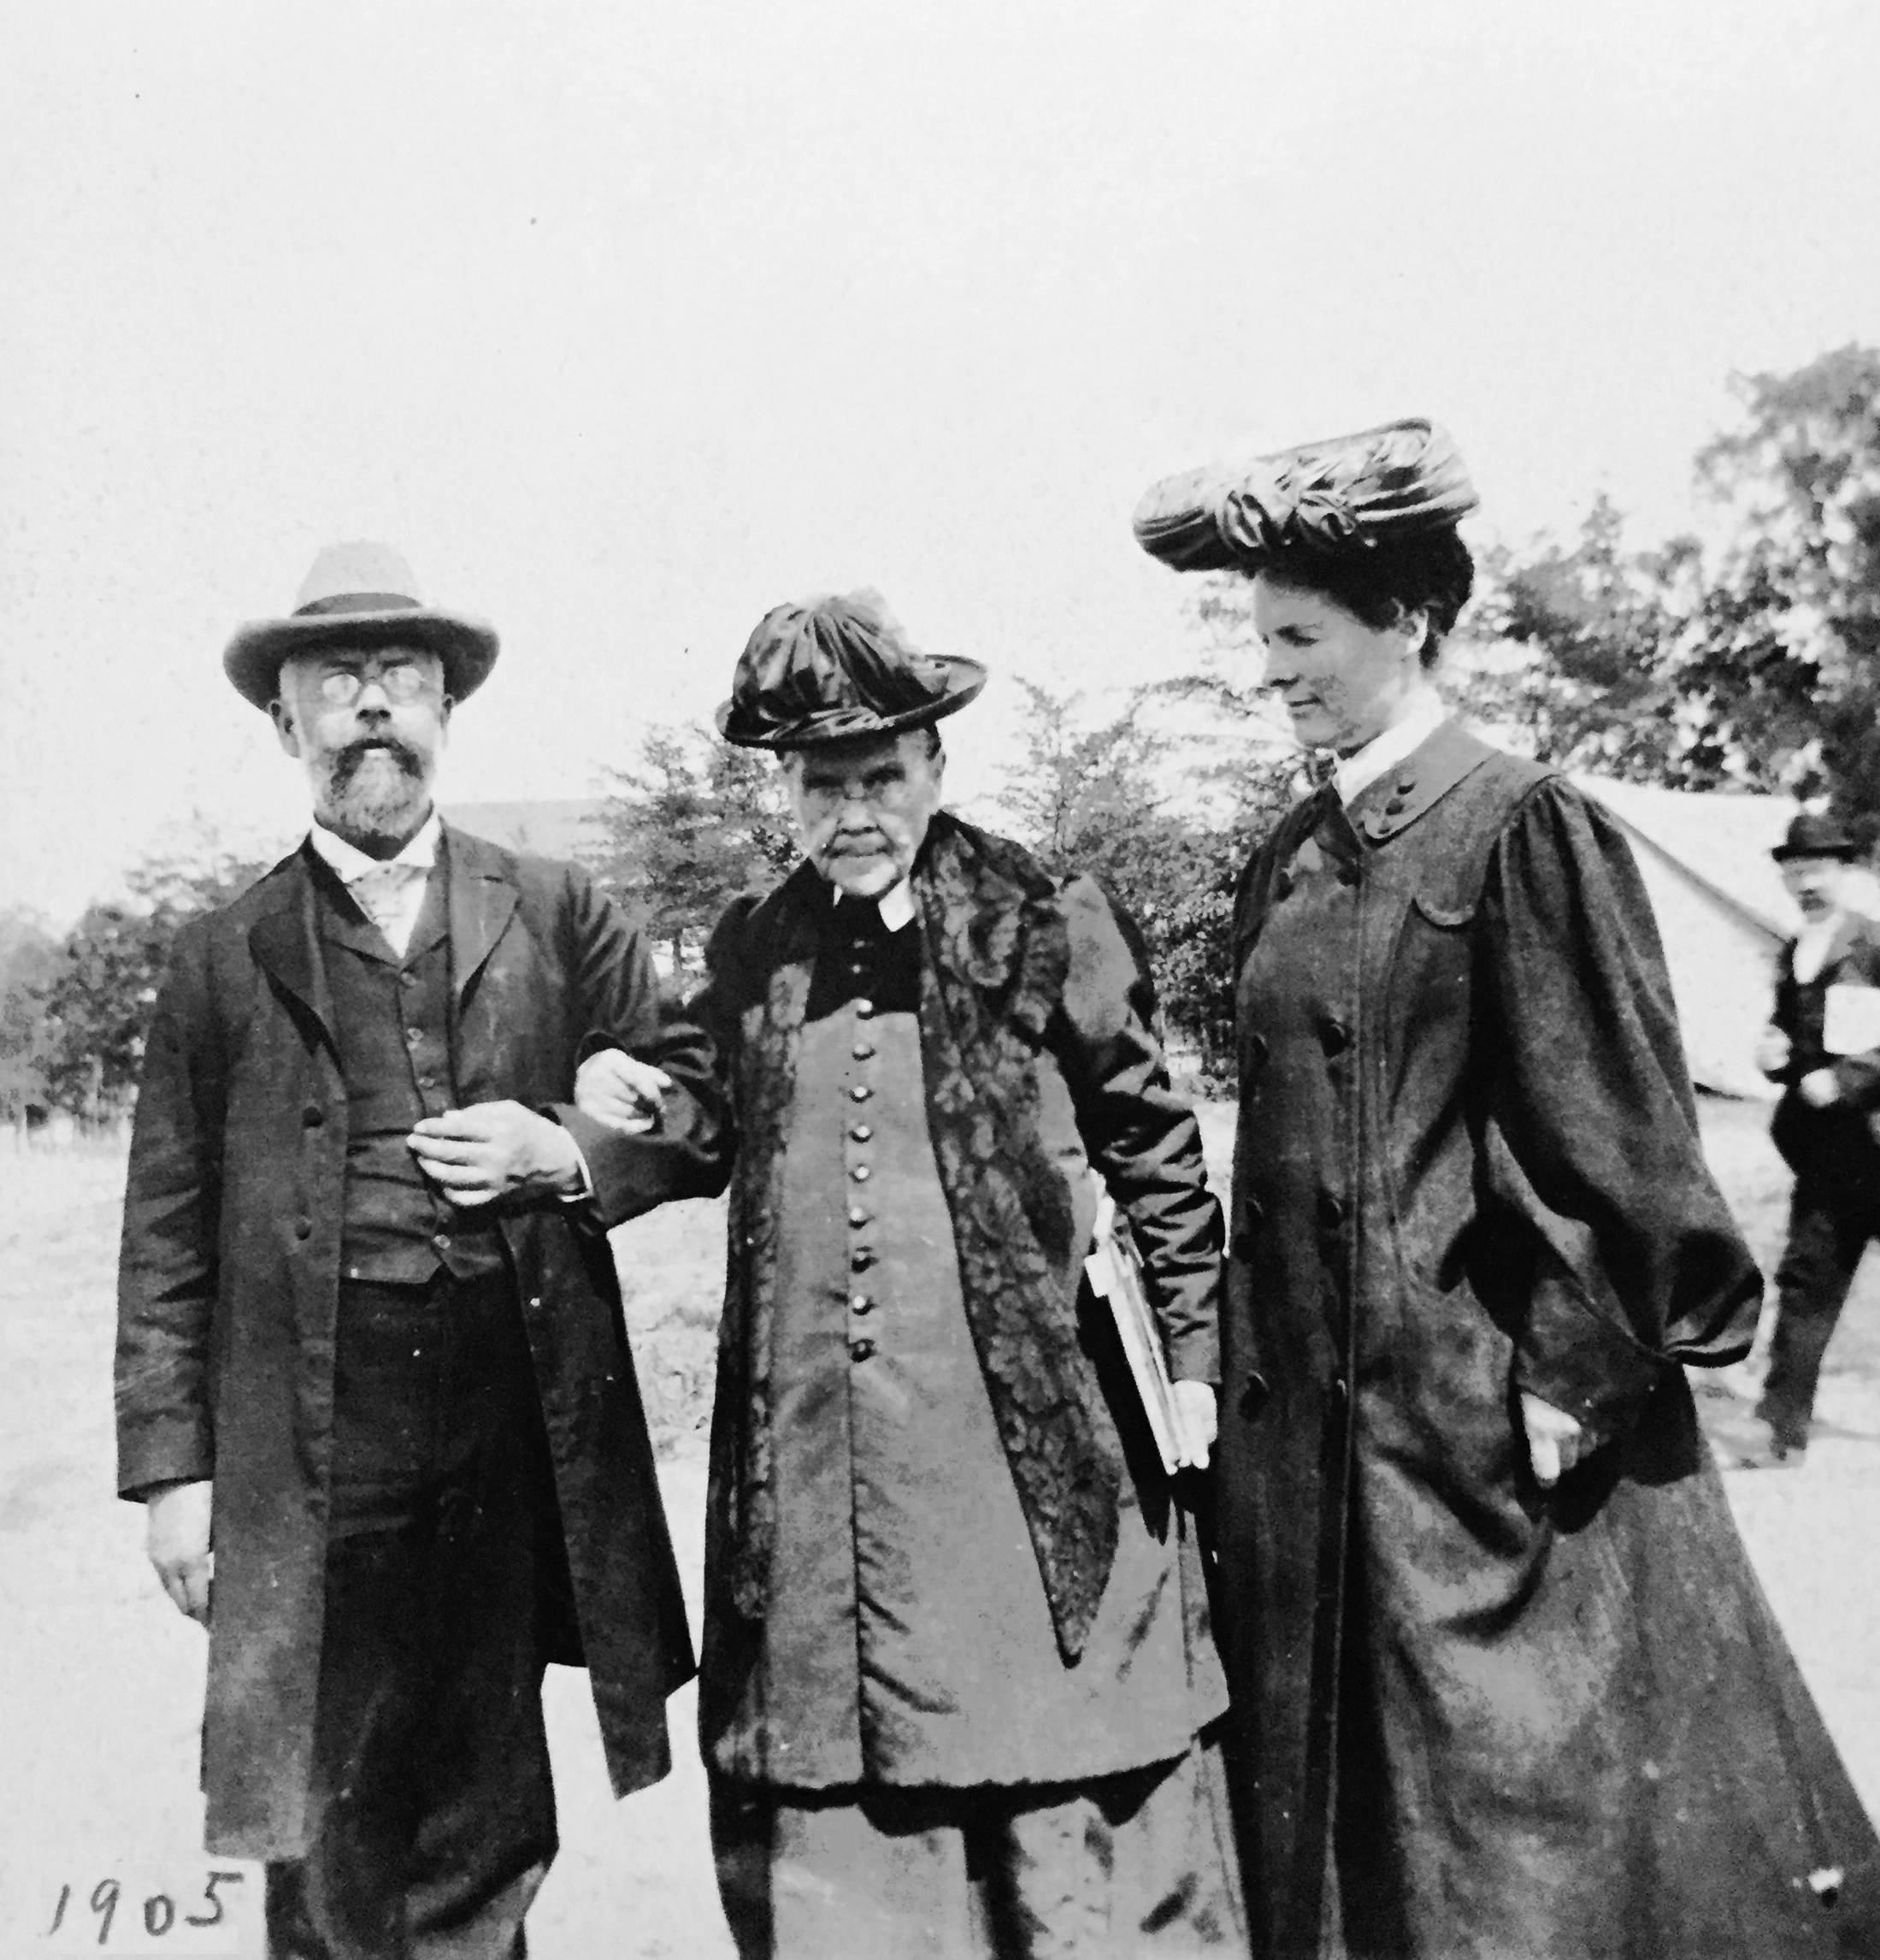
\includegraphics[width=1\linewidth]{images/william-ellen-white-1905.jpg}
    \caption*{William C. White na Ellen G. White, 1905}
    \label{fig:w-e-white}
\end{figure}


According to William White, our only hope as Seventh-day Adventists is to adhere to first principles. These principles, as we know, are the \emcap{Fundamental Principles}. Then, he referred to the order in which the enemy is attacking our work. The attack begins with our disunity, then aims to weaken our reverence for the Sabbath and the Sanctuary service, targets our confidence in the Spirit of Prophecy, and finally focuses on confusing our conceptions regarding personal God.


Kulingana na William White, tumaini letu pekee kama Waadventista Wasabato ni kuzingatia kanuni za kwanza. Kanuni hizi, kama tunavyojua, ni \emcap{Kanuni za Msingi}. Kisha, alitaja kwa mpangilio ambao adui anashambulia kazi yetu. Shambulio linaanza na mifarakano yetu, basi inalenga kudhoofisha heshima yetu kwa Sabato na huduma ya Patakatifu, inalenga imani yetu katika Roho ya Unabii, na hatimaye inalenga kuchanganya dhana zetu kuhusu Mungu wa kibinafsi.


Sister White’s response to William White is of a startling nature. She hints to us that the great apostasy is soon to be realized, and that our hope is to adhere to the first principles of our faith—the \emcap{Fundamental Principles}.


Jibu la Dada White kwa William White ni la asili ya kushangaza. Anatudokezea kuwa ukengeufu mkuu utakuja kutimizwa hivi karibuni, na kwamba tumaini letu ni kuzingatia kanuni za kwanza za imani yetu—\emcap{Kanuni za Msingi}.


\egw{Elmshaven, St. Helena, California} \\
\egw{December 4, 1905} \\
\egw{W. C. White} \\
\egw{My dear son - }


\egw{Elmshaven, St. Helena, California} \\
\egw{Desemba 4, 1905} \\
\egw{W. C. White} \\
\egw{Mwanangu mpendwa - }


\egw{...}


\egw{...}


\egw{“\textbf{One thing it is certain is soon to be realized—\underline{the great apostasy}, which is developing and increasing and waxing stronger and \underline{will continue} to do so until the Lord shall descend from heaven with a shout. \underline{We are to hold fast the first principles of our denominated faith} and go forward from strength to increased faith. \underline{Ever} we are to keep the faith that has been substantiated by the Holy Spirit of God \underline{from the earlier events of our experience until the present time}.} We need now larger breadth and deeper, more earnest, unwavering faith in the leadings of the Holy Spirit. \textbf{If we needed the manifest proof of the Holy Spirit’s power to confirm truth \underline{in the beginning}, after the passing of the time, \underline{we need today all the evidence in the confirmation of the truth}, when souls are departing from the faith and giving heed to seducing spirits and doctrines of devils.} There must not be any languishing of soul now. If ever there was a period of time when we needed the Holy Spirit’s power in our discourses, in our prayers, in every action proposed, it is now. \textbf{We are not to stop at the first experience, but while we bear \underline{the same message} to the people, \underline{this message is to be strengthened and enlarged}}. \textbf{We are to see and realize the importance of the message made certain by its divine origin}. We are to follow on to know the Lord, that we may know that His going forth is prepared as the morning. Our souls need the quickening from the Source of all power. \textbf{We may be strengthened and confirmed in the past experience \underline{that holds us to the essential points of truth which have made us what we are—Seventh-day Adventists}.}“}[Lt326-1905.2; 1905][https://egwwritings.org/read?panels=p7678.8]


\egw{“\textbf{Jambo moja ambalo ni hakika litatimizwa hivi karibuni—\underline{uasi mkubwa}, unaoendelea na kuongezeka na kuzidi kuwa na nguvu na \underline{itaendelea} kufanya hivyo mpaka Bwana atakaposhuka kutoka mbinguni kwa sauti kuu. \underline{Tunapaswa kushika kwa nguvu kanuni za kwanza za imani yetu ya kimadhehebu} na kwenda mbele kutoka nguvu hadi imani iliyoongezeka. \underline{Milele} tunapaswa kuhifadhi imani ambayo imethibitishwa na Roho Mtakatifu wa Mungu tangu awali matukio ya uzoefu wetu hadi wakati huu.} Sasa tunahitaji upana mkubwa zaidi na kina zaidi, imani yenye bidii zaidi, isiyoyumba-yumba katika mwongozo wa Roho Mtakatifu. \textbf{Ikiwa tulihitaji dhihirisho la uthibitisho wa uwezo wa Roho Mtakatifu kuthibitisha ukweli \underline{hapo mwanzo}, baada ya kupita kwa wakati, \underline{tunahitaji leo ushahidi wote katika uthibitisho wa ukweli}, wakati nafsi wanajitenga na imani na kutii roho zidanganyazo na mafundisho ya mashetani.} Ni lazima kusiwe na kudhoofika kwa roho sasa. Ikiwa kulikuwa na kipindi cha wakati tulipohitaji nguvu za Roho Mtakatifu katika mazungumzo yetu, katika maombi yetu, katika kila tendo lililopendekezwa, ni sasa. \textbf{Hatupaswi kuacha uzoefu wa kwanza, lakini wakati tunavumilia \underline{ujumbe huo} kwa watu, \underline{ujumbe huu unapaswa kuimarishwa na kupanuliwa}}. \textbf{Tunapaswa kuona na kutambua umuhimu wa ujumbe unaohakikishwa na asili yake ya kiungu}. Tunapaswa kufuata ili kumjua Bwana, ili tujue kwamba kutoka kwake kumetayarishwa kama vile asubuhi. Nafsi zetu zinahitaji kuhuishwa kutoka kwa Chanzo cha nguvu zote. \textbf{Tunaweza kuimarishwa na kuthibitishwa katika uzoefu uliopita \underline{ambao unatushikilia kwa mambo muhimu ya ukweli ambayo yametufanya tulivyo—Waadventista Wasabato}.}”}[Lt326-1905.2; 1905][https://egwwritings.org/read?panels=p7678.8]


\egwnogap{\textbf{The past fifty years have not dimmed one jot or principle of our faith as we received the great and wonderful evidences that were made certain to us in 1844, after the passing of the time.} The languishing souls are to be confirmed and quickened according to His Word. And many of the ministers of the gospel and the Lord’s physicians will have their languishing souls quickened according to the Word. \textbf{\underline{Not a word is changed or denied}.} \textbf{That which the Holy Spirit testified to as truth after the passing of the time, in our great disappointment, is \underline{the solid foundation of truth}. Pillars of truth were revealed, and we accepted \underline{the foundation principles} that have made us what we are—Seventh-day Adventists, keeping the commandments of God and having the faith of Jesus.}}[Lt326-1905.3; 1905][https://egwwritings.org/read?panels=p7678.9]


\egwnogap{\textbf{Miaka hamsini iliyopita haijafifisha yodi moja au kanuni ya imani yetu kama tulivyopokea ushahidi mkubwa na wa ajabu ambao ulifanywa kuwa hakika kwetu mnamo 1844, baada ya kupita kwa wakati.} Roho zinazodhoofika zinapaswa kuthibitishwa na kuhuishwa kulingana na Neno Lake. Na wengi wa wahudumu wa injili na waganga wa Bwana wao watakuwa na roho zinazodhoofika zilizohuishwa kulingana na Neno. \textbf{\underline{Hakuna neno linalobadilishwa au kukataliwa}.} \textbf{Yale ambayo Roho Mtakatifu alishuhudia kuwa ni kweli baada ya kupita kwa wakati, katika kukatishwa tamaa kuu, ndio \underline{msingi thabiti wa ukweli}. Nguzo za ukweli zilifunuliwa, na tulikubali \underline{kanuni za msingi} ambazo zimetufanya tulivyo—Waadventista Wasabato, wazishikao amri za Mungu na kuwa na imani ya Yesu.}}[Lt326-1905.3; 1905][https://egwwritings.org/read?panels=p7678.9]


This letter is startling because it is an answer to the order of how the enemy is attacking our work. Sister White is well aware of these attacks and she presented the problem in its correct light, also showing us what we shall do to prevent Satan's attacks on us. The enemy wants to \others{confuse our conception regarding a personal God}. This is the very point of great apostasy that \egwinline{is soon to be realized}, and has been \egwinline{developing and increasing and waxing stronger and will continue to do so until the Lord shall descend from heaven with a shout}. This is the apostasy we are experiencing today. What is our hope against this deception and great apostasy? \egwinline{\textbf{\underline{We are to hold fast the first principles of our denominated faith} and go forward from strength to increased faith. \underline{Ever} we are to keep the faith that has been substantiated by the Holy Spirit of God from the earlier events of our experience until the present time.}} \egwinline{...\textbf{\underline{this message is to be strengthened and enlarged}}...} \egwinline{...\textbf{\underline{we need today all the evidence in the confirmation of the truth}}...} \egwinline{\textbf{We may be strengthened and confirmed in the past experience that holds us to the essential points of truth which have made us what we are—Seventh-day Adventists}}. These essential points of truth, which have made us Seventh-day Adventists, are the \emcap{Fundamental Principles}, born in the beginning of our work. In 1905, she wrote, \egwinline{\textbf{The past fifty years have not dimmed one jot or principle of our faith as we received the great and wonderful evidences that were made certain to us in 1844, after the passing of the time.}} \egwinline{\textbf{Not a word is changed or denied.} \textbf{That which the Holy Spirit testified to as truth after the passing of the time, in our great disappointment, is \underline{the solid foundation of truth}. Pillars of truth were revealed, and we accepted \underline{the foundation principles} that have made us what we are—Seventh-day Adventists, keeping the commandments of God and having the faith of Jesus.}}


Barua hii inashangaza kwa sababu ni jibu la mpangilio wa jinsi adui anavyoshambulia kazi yetu. Dada White anafahamu vyema mashambulizi haya na aliwasilisha tatizo hili kwa nuru yake sahihi, pia akituonyesha kile tutakachofanya ili kuzuia mashambulizi ya Shetani juu yetu. Adui anataka \others{kuchanganya dhana yetu kuhusu Mungu wa kibinafsi}. Hii ni hatua ya ukengeufu mkuu ambao \egwinline{utatimizwa hivi karibuni}, na umekuwa \egwinline{ukiendelea na kuongezeka na kuongezeka nguvu zaidi na itaendelea kufanya hivyo mpaka Bwana atakaposhuka kutoka mbinguni pamoja na mwaliko}. Huu ndio ukengeufu tunaoupata leo. Nini matumaini yetu dhidi ya udanganyifu huu na uasi mkuu? \egwinline{\textbf{\underline{Tunapaswa kushikilia kwa dhati kanuni za kwanza za imani yetu ya kimadhehebu} na kwenda mbele kutoka kwa nguvu hadi imani iliyoongezeka. \underline{Daima} tunapaswa kutunza imani yetu ambayo imethibitishwa na Roho Mtakatifu wa Mungu kutokana na matukio ya awali ya uzoefu wetu mpaka wakati huu.}} \egwinline{...\textbf{\underline{ujumbe huu unapaswa kuimarishwa na kukuzwa}}...} \egwinline{...\textbf{\underline{tunahitaji leo ushahidi wote katika uthibitisho wa ukweli}}...} \egwinline{\textbf{Tunaweza kuimarishwa na kuthibitishwa katika uzoefu uliopita ambao unatushikilia kwa muhimu mambo ya ukweli ambayo yametufanya tuwe hivi tulivyo—Waadventista Wasabato}}. Haya mambo muhimu ya ukweli, ambayo yametufanya sisi Waadventista Wasabato, ndiyo \emcap{Kanuni za Kimsingi}, zilizozaliwa mwanzoni mwa kazi yetu. Mnamo 1905, aliandika, \egwinline{\textbf{Miaka hamsini iliyopita haijafifisha yodi moja au kanuni ya imani yetu kama tulivyopokea ushahidi mkubwa na wa ajabu ambao ulifanywa kuwa hakika kwetu mnamo 1844, baada ya kupita kwa wakati.}} \egwinline{\textbf{\underline{Hakuna neno linalobadilishwa au kukataliwa}.} \textbf{Yale ambayo Roho Mtakatifu alishuhudia kuwa ni kweli baada ya kupita kwa wakati, katika kukatishwa tamaa kuu, ndio \underline{msingi thabiti wa ukweli}. Nguzo za ukweli zilifunuliwa, na tulikubali \underline{kanuni za msingi} ambazo zimetufanya tulivyo—Waadventista Wasabato, wazishikao amri za Mungu na kuwa na imani ya Yesu.}}


God calls us to be steadfast in the \emcap{Fundamental Principles}, especially over the \others{conception regarding a personal God}. This is the first point of the \emcap{Fundamental Principles}.


Mungu anatuita kuwa imara katika \emcap{Kanuni za Kimsingi}, hasa juu ya \others{dhana kuhusu Mungu binafsi}. Hili ni jambo la kwanza la \emcap{Kanuni za Kimsingi}.


Sister White foretold that a great apostasy is developing in our church regarding the understanding of the \emcap{personality of God}. The true understanding of the \emcap{personality of God} is presented in the \emcap{Fundamental Principles}. She clearly warned us of Satan’s attack on these principles. She calls us to \egw{\textbf{hold fast the first principles of our denominated faith} and go forward from strength to increased faith}.


Dada White alitabiri kwamba ukengeufu mkubwa unaendelea katika kanisa letu kuhusu ufahamu wa \emcap{Umbile la Mungu}. Ufahamu wa kweli wa \emcap{Umbile la Mungu} umewasilishwa katika \emcap{Kanuni za Kimsingi}. Alituonya waziwazi kuhusu shambulio la Shetani dhidi ya kanuni hizi. Anatuita \egw{\textbf{kushikilia sana kanuni za kwanza za imani yetu ya kimadhehebu} na kwenda mbele kutoka nguvu hadi imani iliyoongezeka}.


\egw{\textbf{“After the passing of the time, God entrusted to His faithful followers the precious \underline{principles of present truth}. These principles were not given to those who had had no part in the giving of the first and second angels’ messages. They were given to the workers who had had a part in the cause from the beginning}.”}[Ms129-1905.5; 1905][https://egwwritings.org/read?panels=p9797.12]


\egw{\textbf{“Baada ya muda kupita, Mungu aliwakabidhi wafuasi Wake waaminifu vitu vya thamani \underline{kanuni za ukweli wa sasa}. Kanuni hizi hazikutolewa kwa wale ambao hawakuwa na sehemu katika utoaji wa ujumbe wa malaika wa kwanza na wa pili. Walipewa kwa wafanyakazi ambao walikuwa na sehemu katika kazi hiyo tangu mwanzo}.”}[Ms129-1905.5; 1905][https://egwwritings.org/read?panels=p9797.12]


\egwnogap{\textbf{Those who passed through these experiences are to be as \underline{firm as a rock to the principles} that have made us Seventh-day Adventists}. They are to be workers together with God, binding up the testimony and sealing the law among His disciples. Those who took part in the establishment of our work upon the foundation of Bible truth; \textbf{those who know the waymarks that have pointed out the right path} are to be regarded as workers of the highest value. They can speak from personal experience, regarding the truths entrusted to them. These men are not to permit their faith to be changed to infidelity; they are not to permit the banner of the third angel to be taken from their hands. They are to hold the beginning of their confidence firm unto the end. \textbf{\underline{The Lord has declared that the history of the past shall be rehearsed as we enter upon the closing work}. Every truth that He has given for these last days is to be proclaimed to the world. \underline{Every pillar} that He has established \underline{is to be strengthened}. We cannot now step off the foundation that God has established. We cannot now enter into any new organization; for this would mean apostasy from the truth}.}[Ms129-1905.6; 1905][https://egwwritings.org/read?panels=p9797.13]


\egwnogap{\textbf{Wale ambao walipitia uzoefu huu wanapaswa kuwa \underline{thabiti kama mwamba kwa kanuni} ambazo zimetufanya kuwa Waadventista Wasabato}. Wanapaswa kuwa wafanyakazi pamoja na Mungu, akifunga ushuhuda na kutia muhuri sheria kati ya wanafunzi wake. Wale waliochukua sehemu katika kusimamisha kazi yetu juu ya msingi wa kweli ya Biblia; \textbf{wale wanaojua viashiria njia ambavyo vimeonyesha njia sahihi} wanapaswa kuzingatiwa kama wafanyikazi wa thamani ya juu. Wanaweza kusema kutokana na uzoefu wa kibinafsi, kuhusu kweli walizokabidhiwa wao. Watu hawa hawapaswi kuruhusu imani yao ibadilishwe na kuwa ukafiri; hawatakiwi kuruhusu bendera ya malaika wa tatu kuchukuliwa kutoka mikononi mwao. Wanapaswa kushikilia mwanzo wa imani yao imara hadi mwisho. \textbf{\underline{Bwana ametangaza kwamba historia iliyopita itarudiwa tunapoingia kwenye kazi ya utimisho}. Kila ukweli alionao iliyotolewa kwa ajili ya siku hizi za mwisho itatangazwa kwa ulimwengu. \underline{Kila nguzo} imara aliyotengeneza \underline{itaimarishwa}. Hatuwezi sasa kuondoa kwa msingi ambao Mungu ameanzisha. Hatuwezi sasa kuingia katika shirika lolote jipya; kwa maana hii ni kuasi kutoka kwa ukweli}.}[Ms129-1905.6; 1905][https://egwwritings.org/read?panels=p9797.13]


Stepping off of the foundation that God has established means entering into new organization; this is apostasy from the truth. Comparing the \emcap{Fundamental Principles} of the past with current trinitarian Fundamental Beliefs, it’s evident we’re in a state of apostasy.  Ellen White prophesied that this apostasy will be \egwinline{\textbf{developing and increasing and waxing stronger and \underline{will continue} to do so until the Lord shall descend from heaven with a shout}}[Lt326-1905.2; 1905][https://egwwritings.org/read?panels=p7678.8].


Kuondoka kwenye msingi ambao Mungu ameweka kunamaanisha kuingia katika shirika jipya; huu ni ukengeufu kutoka kwa ukweli. Kulinganisha \emcap{Kanuni za Kimsingi} za zamani na Imani za Msingi za utatu wa sasa, ni dhahiri tuko katika hali ya ukengeufu. Ellen White alitabiri kwamba ukengeufu huu utakuwa \egwinline{\textbf{ukiendelea na kuongezeka na kukua kwa nguvu zaidi na \underline{itaendelea} kufanya hivyo hadi Bwana atakaposhuka kutoka mbinguni kwa ukemi}}[Lt326-1905.2; 1905][https://egwwritings.org/read?panels=p7678.8].


% The great apostasy is soon to be realized

\begin{titledpoem}
    
    \stanza{
        In a letter penned, a crisis foretold, \\
        From Ellen White, a warning bold: \\
        "Adhere to the roots of our Adventist comprehend, \\
        For soon will come apostasy's seed."
    }

    \stanza{
        The pillars strong of our founding year, \\
        Are under siege, as Ellen feared. \\
        To "Meet it!" was her stern command, \\
        To hold the line, to firmly stand.
    }

    \stanza{
        "Keep to the principles," her urgent plea, \\
        From 1844's prophetic decree. \\
        For truth confirmed by the Spirit's flame, \\
        Shall not be denied, nor put to shame.
    }

    \stanza{
        The enemy seeks to divide and sway, \\
        To change our course, to lead astray. \\
        But steadfast hearts must ever cling \\
        To the first truths that made our spirits sing.
    }

    \stanza{
        Hold fast, she wrote, to what we know, \\
        The Fundamental Principles that show \\
        The way to live, the path to trod, \\
        Under the gaze of an unchanging God.
    }

    \stanza{
        For as the world spins toward its close, \\
        The truth of Ellen White still glows— \\
        A beacon strong against the night, \\
        Guiding the faithful in the right.
    }
    
\end{titledpoem}


% The great apostasy is soon to be realized

\begin{titledpoem}
    
    \stanza{
        In a letter penned, a crisis foretold, \\
        From Ellen White, a warning bold: \\
        "Adhere to the roots of our Adventist comprehend, \\
        For soon will come apostasy's seed."
    }

    \stanza{
        The pillars strong of our founding year, \\
        Are under siege, as Ellen feared. \\
        To "Meet it!" was her stern command, \\
        To hold the line, to firmly stand.
    }

    \stanza{
        "Keep to the principles," her urgent plea, \\
        From 1844's prophetic decree. \\
        For truth confirmed by the Spirit's flame, \\
        Shall not be denied, nor put to shame.
    }

    \stanza{
        The enemy seeks to divide and sway, \\
        To change our course, to lead astray. \\
        But steadfast hearts must ever cling \\
        To the first truths that made our spirits sing.
    }

    \stanza{
        Hold fast, she wrote, to what we know, \\
        The Fundamental Principles that show \\
        The way to live, the path to trod, \\
        Under the gaze of an unchanging God.
    }

    \stanza{
        For as the world spins toward its close, \\
        The truth of Ellen White still glows— \\
        A beacon strong against the night, \\
        Guiding the faithful in the right.
    }
    
\end{titledpoem}
